\documentclass[a4paper,12pt]{article}
\usepackage[cm]{fullpage}
\usepackage{url}
\usepackage{xcolor}
\usepackage{graphicx}
\usepackage{amsmath}
\usepackage{amsfonts}
\usepackage{upgreek}
\usepackage{bm}
\usepackage{listings}
\usepackage{tikz}
\usepackage{siunitx}

\lstset{ 
  language=Python,
  backgroundcolor=\color{white},   % choose the background color; you must add \usepackage{xcolor}; should come as last argument
  basicstyle=\footnotesize,        % the size of the fonts that are used for the code
  breakatwhitespace=false,         % sets if automatic breaks should only happen at whitespace
  breaklines=true,                 % sets automatic line breaking
  captionpos=b,                    % sets the caption-position to bottom
  frame=single,                    % adds a frame around the code
  keepspaces=true,                 % keeps spaces in text, useful for keeping indentation of code 
  keywordstyle=\color{blue},       % keyword style
}

\usetikzlibrary{arrows, arrows.meta}

\bibliographystyle{plain} % We choose the "plain" reference style

\newcommand{\nn}{\nonumber}
\newcommand{\captionfont}{\tiny}
\newcommand{\QtwoQone}{$Q_2\times Q_1$}
\newcommand{\python}{\color{teal} \sffamily }
\newcommand{\K}{{\mathbb{K}}}
\newcommand{\G}{{\mathbb{G}}}

%%%%%%%%%%%%%%%%%%%%%%%%%%%%%%%%%%%%%%%%%%%%%%%%%%%%%%%%%%%%%%%%%%%%%%%%%%%%%%%
%%%%%%%%%%%%%%%%%%%%%%%%%%%%%%%%%%%%%%%%%%%%%%%%%%%%%%%%%%%%%%%%%%%%%%%%%%%%%%%
%%%%%%%%%%%%%%%%%%%%%%%%%%%%%%%%%%%%%%%%%%%%%%%%%%%%%%%%%%%%%%%%%%%%%%%%%%%%%%%
%%%%%%%%%%%%%%%%%%%%%%%%%%%%%%%%%%%%%%%%%%%%%%%%%%%%%%%%%%%%%%%%%%%%%%%%%%%%%%%
%%%%%%%%%%%%%%%%%%%%%%%%%%%%%%%%%%%%%%%%%%%%%%%%%%%%%%%%%%%%%%%%%%%%%%%%%%%%%%%
\begin{document}
\title{FLAPS \\ the FLexible Axisymmetric Planet Solver}
\author{C. Thieulot}
\maketitle

\begin{center}
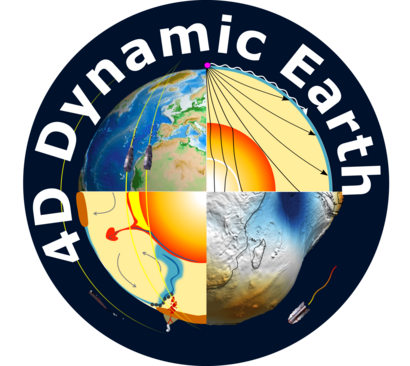
\includegraphics[width=5cm]{images/4DDynamicEarth}
\end{center}

%%%%%%%%%%%%%%%%%%%%%%%%%%%%%%%%%%%%%%%%%%%%%%%%%%%%%%%%%%%%%%%%%%%%%%%%%%%%%%%
\newpage
\section{Introduction}

This code first started as a stone in the fieldstone project \cite{fieldstone}.
As it was growing and it appeared that it would be used for different projects
I decided to take it out and turn it into a standalone code with its own manual.

The code only supports one type of Finite Elements, the $Q_2\times Q_1$ pair, 
which is stable and commonly used in geodynamics \ref{thba22}.

%%%%%%%%%%%%%%%%%%%%%%%%%%%%%%%%%%%%%%%%%%%%%%%%%%%%%%%%%%%%%%%%%%%%%%%%%%%%%%%
\newpage
\section{The physics}


The domain is a spherical shell centered around the origin of the Cartesian 
axis system $(x,y,z)$. 
The inner radius is denoted by $R_1$ and the outer radius by $R_2$.
The Stokes equations are solved in the domain and the flow is assumed 
to be instantaneous, incompressible and isothermal.

The velocity in Cartesian coordinates is denoted by $\vec{v}=(v_x,v_y,v_z)$ and 
$\vec{v}=(v_r,v_\theta,v_\phi)$ in spherical coordinates. 
The equations to solve are then

\begin{eqnarray}
- \vec\nabla p + \vec\nabla \cdot (2 \eta \dot{\bm \varepsilon}(\vec v))  + \rho \vec{g} &=& 0 \\
\vec\nabla \cdot \vec{v} &=& 0
\end{eqnarray}
The domain has two boundaries: the inner boundary $r=R_1$ and the outer boundary at $r=R_2$.
Boundary conditions can be either no slip, free slip or open ('free surface').

The domain is filled with a fluid (the mantle 'm') of viscosity $\eta_m(\vec{r})$ 
and density $\rho_m(\vec{r})$.
A sphere ('s') of a different fluid or radius $R_s$ is placed at location $(0,0,z_s)$ with 
viscosity $\eta_s$ and density $\rho_s$. As such the setup is 
axisymmetric along the North-South poles line.
The gravity $\vec{g}=-g \vec{e}_r$ points towards the center of the shell\footnote{unless 
self gravitation is used}.

\begin{center}
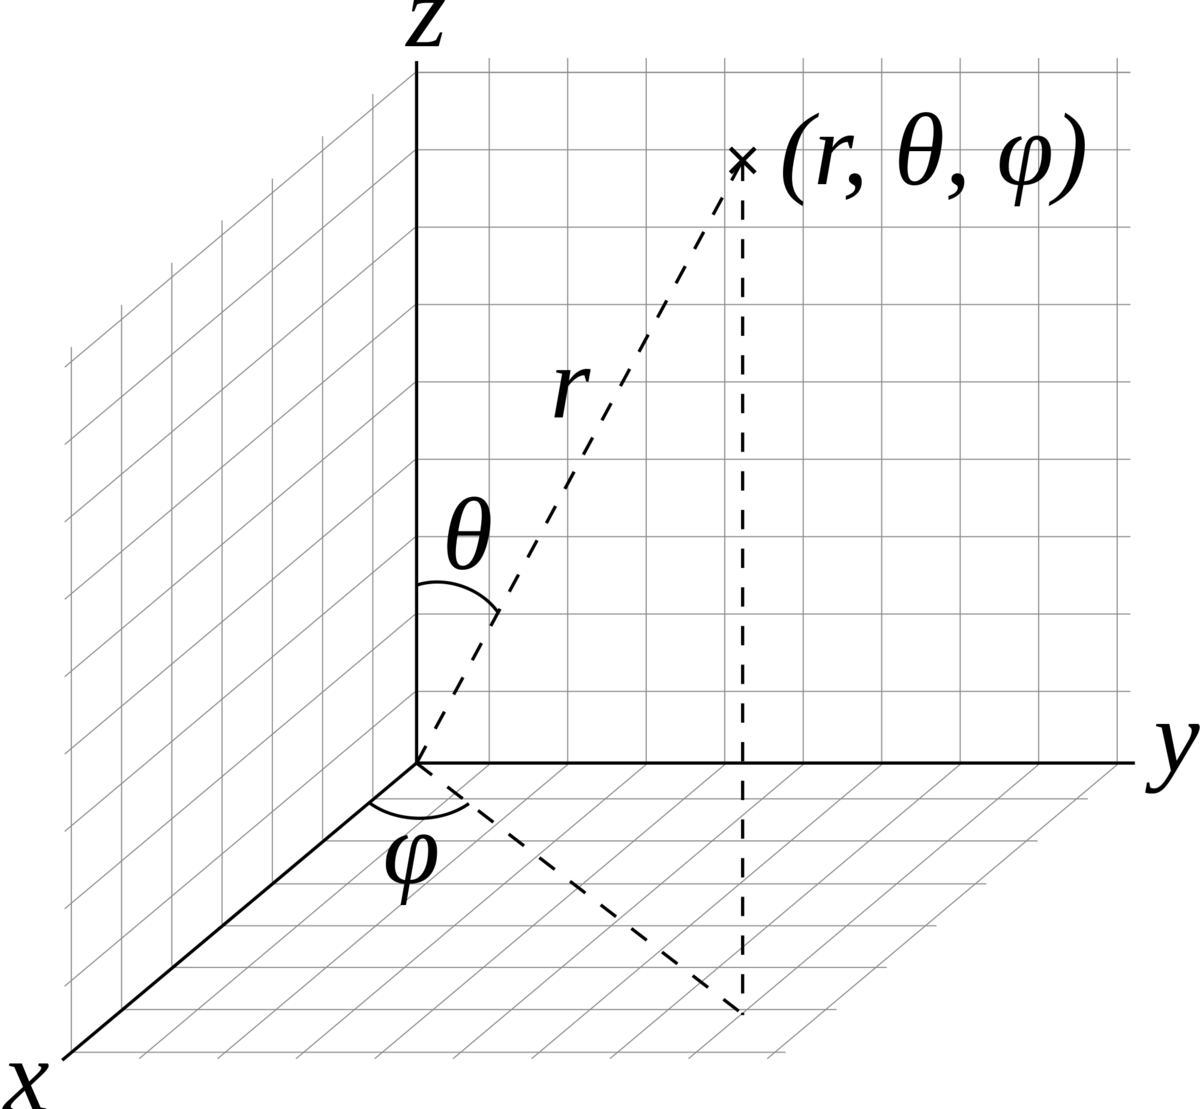
\includegraphics[width=6.5cm]{images/sphcoord}
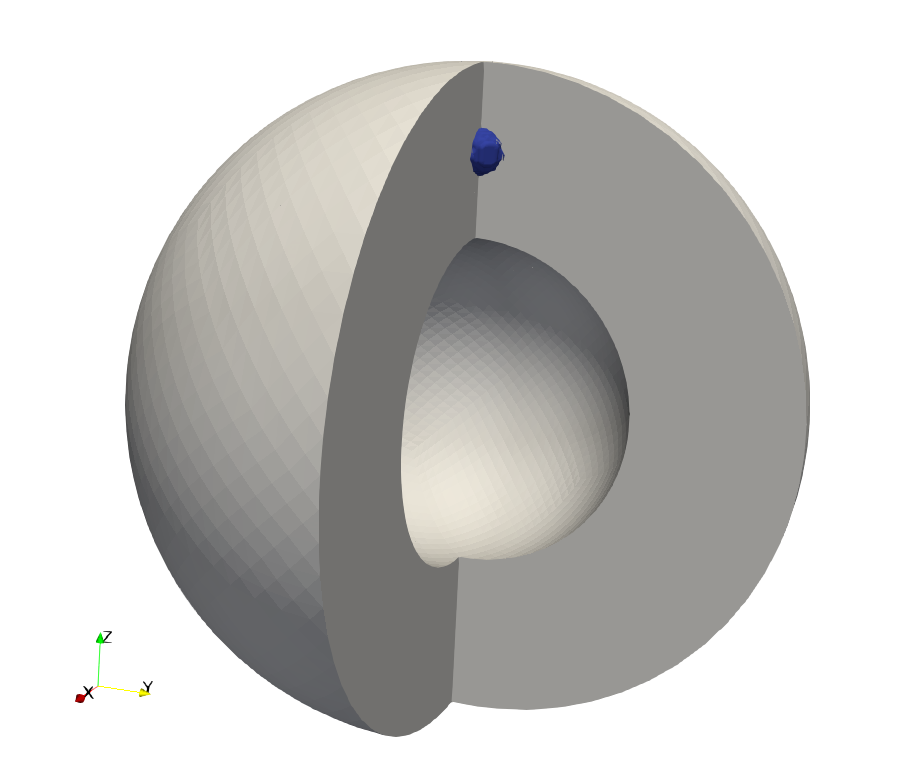
\includegraphics[width=8cm]{images/setup}
\end{center}

Models with free slip boundary conditions on both inner and outer surfaces have a rotational nullspace which needs to be removed. 

In such case the pressure also showcases a constant value nullspace which can be removed by ensuring that the average surface pressure is zero.


%----------------------------------------------------------
\subsection{About the gravity field}

We need to specify the gravity acceleration vector $\vec{g}$
inside the domain. 
We have several option. 

\begin{itemize}
\item the simplest option is to set $\vec{g} = - g_0 \vec{e}_r$
with $g_0$ being a constant (e.g. 9.8~\si{\meter\per\second}).
This is {\python gravity\_model=0}


\item We can assume the domain to be spherically symmetric: 
the core has a density $\rho_c$ and the mantle has a density $\rho_m$.
In that case we have
In the end we have:
\begin{eqnarray}
g_c(r)&=& \frac{1}{3}\hat{\rho}_c r \nn\\ 
g_m(r)&=& \frac{1}{3}\hat{\rho}_m r +\frac{C}{r^2} 
\end{eqnarray}
with 
\[
C=\frac{R_1^3}{3} (\hat{\rho}_c-\hat{\rho}_m)
\]
In the core we have $\vec{g}_c = - g_c(r) \vec{e}_r$
and in the mantle  $\vec{g}_m = - g_m(r) \vec{e}_r$.

\begin{center}
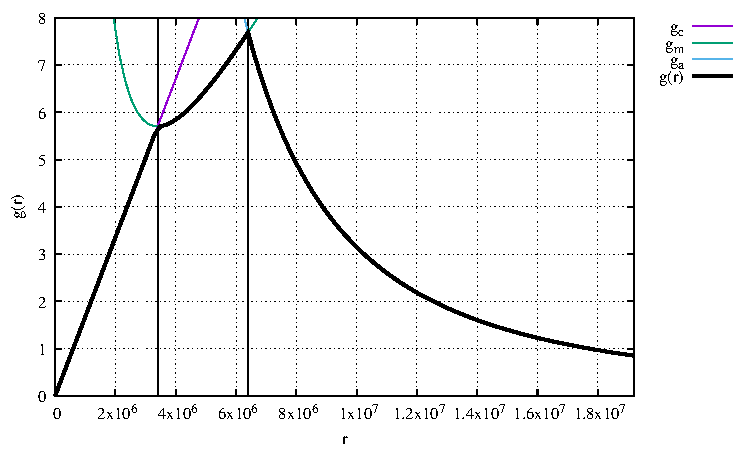
\includegraphics[width=8cm]{images/bench/g}
\end{center}

This is {\python gravity\_model=1}

\item This is no more an axisymmetric case. We have the same 
structure (core and mantle) but there is now a sphere ('blob')
of density $\rho_{blob}$ at location $x=0$ $z=z_{blob}$ of 
radius $R_{blob}$. 

The gravity field is then the sum of the spherically symmetric one 
above and the one generated by the density anomaly in the blob.

This is {\python gravity\_model=2}

\end{itemize}



%----------------------------------------------------------
\subsection{Axisymmetric formulation}


We here rely on axisymmetric cylindrical coordinates, see Section~\ref{MMM-ss:axicyleqs}.
As shown on the following figure we assume that the deformation/flow is independent of the angle 
$\theta$ so that the remaining space coordinates are $r$ and $z$.
\begin{center}
\begin{flushright} {\tiny {\color{gray} (tikz\_axi.tex)}} \end{flushright}
%~~~~~~~~~~~~~~~~~~~~~~~~~~~~~~~~~~~~~~~~~~~~~~~~~~~~~~~~~~~~~~~~~~~~~~~~~~~~~~~~~~~~~~~~~~~~~~~~~~

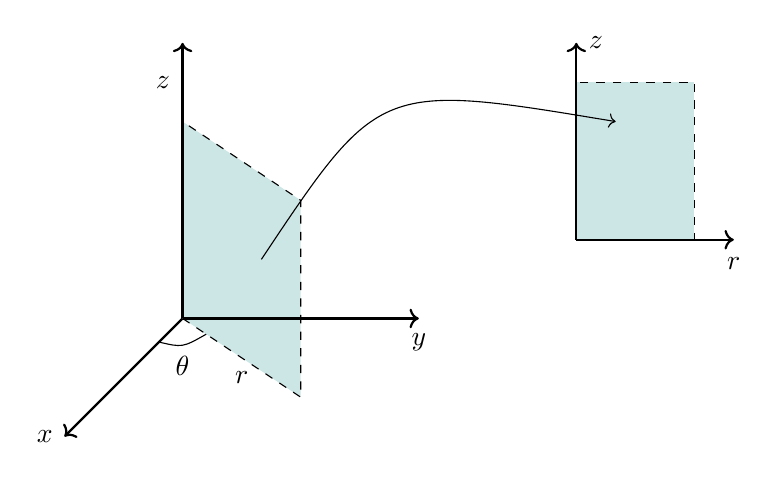
\begin{tikzpicture}
%\draw[step=0.5cm,gray,very thin] (0,0) grid (10,6); %background grid

\draw[dashed,fill=teal!20] (2,2)--(3.5,1)--(3.5,3.5)--(2,4.5)--cycle ;
\draw[thick,->] (2,2) -- (0.5,0.5); 
\draw[thick,->] (2,2) -- (5,2); 
\draw[thick,->] (2,2) -- (2,5.5); 
\node[] at (0.25,0.5) {$x$};
\node[] at (5,1.7) {$y$};
\node[] at (1.75,5) {$z$};
\node[] at (2.75,1.25) {$r$};
\node[] at (2,1.4) {$\theta$};
\draw[] (1.7,1.7) .. controls (2,1.63) ..   (2.3,1.8);

\draw[dashed,fill=teal!20] (7,3)--(8.5,3)--(8.5,5)--(7,5)--cycle; 
\draw[thick,->] (7,3) -- (9,3); 
\draw[thick,->] (7,3) -- (7,5.5); 
\node[] at (9,2.7) {$r$};
\node[] at (7.25,5.5) {$z$};

\draw[->] (3,2.75) .. controls (4.5,5) .. (7.5,4.5);
\end{tikzpicture}



\end{center}

Given the symmetry of the problem any term containing $\partial_\theta$ or $\upnu_\theta$ is zero.
The strain rate tensor given in Section~\ref{MMM-ss:srcc} then simplifies to:

\begin{eqnarray}
\dot\varepsilon_{rr} 
&=& \frac{\partial \upnu_r}{\partial r} \nn\\
\dot\varepsilon_{\theta\theta}  &=& \frac{\upnu_r}{r} \nn\\
\dot\varepsilon_{\theta r} = \dot\varepsilon_{r\theta}  &=& 0 \nn\\
\dot\varepsilon_{zz} &=& \frac{\partial \upnu_z}{\partial z} \nn\\
\dot{\varepsilon}_{rz} = \dot{\varepsilon}_{zr} 
&=& \frac{1}{2}\left( \frac{\partial \upnu_r}{\partial z} + \frac{\partial \upnu_z}{\partial r} \right) \nn\\
\dot{\varepsilon}_{\theta z} = \dot{\varepsilon}_{z \theta} &=& 0 \nn
\end{eqnarray}
or,
\[
\dot{\bm\varepsilon}(\vec\upnu)
=
\left(
\begin{array}{ccc}
\dot\varepsilon_{rr} & 0 & \dot{\varepsilon}_{rz} \\
0 & \dot{\varepsilon}_{\theta\theta}  & 0 \\
\dot{\varepsilon}_{zr} & 0 & \dot\varepsilon_{zz}
\end{array}
\right)
\]
Note that the term $\dot\varepsilon_{\theta\theta} $ is not zero!
The deviatoric stress tensor ${\bm \tau}=2\eta \dot{\bm \varepsilon}$ can be computed
as well as the full stress tensor ${\bm \sigma}=-p {\bm 1} + {\bm \tau}$. 




%----------------------------------------------------------
\subsection{Tensors from Cartesian to Spherical coordinates}
In order to compute the dynamic topography we will need $\sigma_{rr}$, 
which in fact will require $\dot{\varepsilon}_{rr}$. This means that 
having obtained the strain rate tensor in Cartesian coordinates we must 
rewrite it in spherical coordinates with the following conventions:

\begin{center}
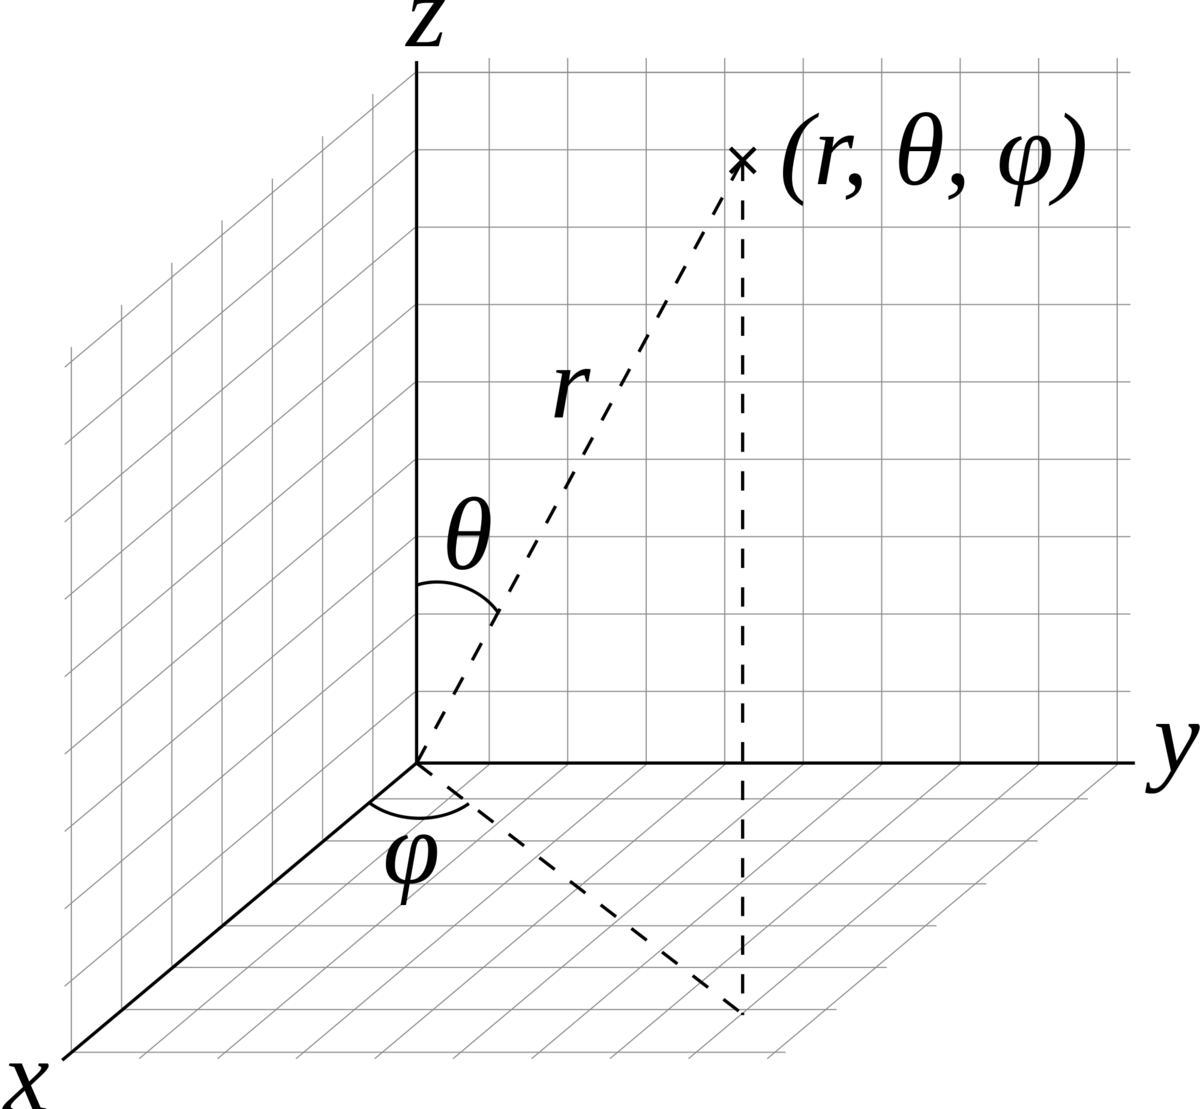
\includegraphics[width=3cm]{images/sphcoord}
\end{center}

We have
\begin{eqnarray}
{\bm T}_{\tiny Sph}&=&
\left(
\begin{array}{ccc}
T_{rr}       & T_{r\theta}      & T_{r\phi} \\
T_{\theta r} & T_{\theta\theta} & T_{\theta\phi} \\
T_{\phi r}   & T_{\phi \theta}  & T_{\phi\phi}
\end{array}
\right) \nn\\
&=&
\left(
\begin{array}{ccc}
\sin\theta \cos\phi & \sin\theta \sin\phi & \cos\theta \\
\cos\theta \cos\phi & \cos\theta \sin\phi & -\sin\theta \\
-\sin\phi & \cos\phi & 0 
\end{array}
\right)
\cdot
\left(
\begin{array}{ccc}
T_{xx} & T_{xy} & T_{xz} \\
T_{yx} & T_{yy} & T_{yz} \\
T_{zx} & T_{zy} & T_{zz} 
\end{array}
\right)
\cdot
\left(
\begin{array}{ccc}
\sin\theta\cos\phi & \cos\theta\cos\phi & -\sin\phi \\
\sin\theta\sin\phi & \cos\theta\sin\phi & \cos\phi \\
\cos\theta & -\sin\theta & 0
\end{array}
\right) 
\nn\\
{\bm T}_{\tiny Cart} &=&
\left(
\begin{array}{ccc}
T_{xx} & T_{xy} & T_{xz} \\
T_{yx} & T_{yy} & T_{yz} \\
T_{zx} & T_{zy} & T_{zz} 
\end{array}
\right) \nn\\
&=&
\left(
\begin{array}{ccc}
\sin\theta\cos\phi & \cos\theta\cos\phi & -\sin\phi \\
\sin\theta\sin\phi & \cos\theta\sin\phi & \cos\phi \\
\cos\theta & -\sin\theta & 0
\end{array}
\right)
\cdot
\left(
\begin{array}{ccc}
T_{rr}       & T_{r\theta}      & T_{r\phi} \\
T_{\theta r} & T_{\theta\theta} & T_{\theta\phi} \\
T_{\phi r}   & T_{\phi \theta}  & T_{\phi\phi}
\end{array}
\right)
\cdot
\left(
\begin{array}{ccc}
\sin\theta \cos\phi & \sin\theta \sin\phi & \cos\theta \\
\cos\theta \cos\phi & \cos\theta \sin\phi & -\sin\theta \\
-\sin\phi & \cos\phi & 0 
\end{array}
\right) \nonumber
\end{eqnarray}
In our case, calculations take place in the 
$(x,z)$-plane so we have $\phi=0$ and the equation above 
becomes
\[
\left(
\begin{array}{ccc}
T_{rr}       & T_{r\theta}      & T_{r\phi} \\
T_{\theta r} & T_{\theta\theta} & T_{\theta\phi} \\
T_{\phi r}   & T_{\phi \theta}  & T_{\phi\phi}
\end{array}
\right)
=
\left(
\begin{array}{ccc}
\sin\theta  & 0 & \cos\theta \\
\cos\theta  & 0 & -\sin\theta \\
0 & 1 & 0 
\end{array}
\right)
\cdot
\left(
\begin{array}{ccc}
T_{xx} & T_{xy} & T_{xz} \\
T_{yx} & T_{yy} & T_{yz} \\
T_{zx} & T_{zy} & T_{zz} 
\end{array}
\right)
\cdot
\left(
\begin{array}{ccc}
\sin\theta & \cos\theta & 0 \\
0 & 0 & 1 \\
\cos\theta & -\sin\theta & 0
\end{array}
\right)
\]
We define $c_\theta=\cos\theta$, $s_\theta=\sin\theta$ so that
\[
\left(
\begin{array}{ccc}
T_{rr}       & T_{r\theta}      & T_{r\phi} \\
T_{\theta r} & T_{\theta\theta} & T_{\theta\phi} \\
T_{\phi r}   & T_{\phi \theta}  & T_{\phi\phi}
\end{array}
\right)
=
\left(
\begin{array}{ccc}
s_\theta  & 0 & c_\theta \\
c_\theta  & 0 & -s_\theta \\
0 & 1 & 0 
\end{array}
\right)
\cdot
\left(
\begin{array}{ccc}
T_{xx} & T_{xy} & T_{xz} \\
T_{yx} & T_{yy} & T_{yz} \\
T_{zx} & T_{zy} & T_{zz} 
\end{array}
\right)
\cdot
\left(
\begin{array}{ccc}
s_\theta & c_\theta & 0 \\
0 & 0 & 1 \\
c_\theta & -s_\theta & 0
\end{array}
\right)
\]
As we have seen above we have 
\[
\dot{\bm\varepsilon}_{\tiny Cart}
=
\left(
\begin{array}{ccc}
\dot\varepsilon_{xx} & 0 & \dot{\varepsilon}_{xz} \\
0 & \dot{\varepsilon}_{yy}  & 0 \\
\dot{\varepsilon}_{xz} & 0 & \dot\varepsilon_{zz}
\end{array}
\right)
\]
so 
\begin{eqnarray}
\dot{\bm \varepsilon}_{\tiny Sph}=
\left(
\begin{array}{ccc}
\dot\varepsilon_{rr}       & \dot\varepsilon_{r\theta}      & \dot\varepsilon_{r\phi} \\
\dot\varepsilon_{\theta r} & \dot\varepsilon_{\theta\theta} & \dot\varepsilon_{\theta\phi} \\
\dot\varepsilon_{\phi r}   & \dot\varepsilon_{\phi \theta}  & \dot\varepsilon_{\phi\phi}
\end{array}
\right)
&=&
\left(
\begin{array}{ccc}
s_\theta  & 0 & c_\theta \\
c_\theta  & 0 & -s_\theta \\
0 & 1 & 0 
\end{array}
\right)
\cdot
\left(
\begin{array}{ccc}
\dot\varepsilon_{xx} & 0 & \dot{\varepsilon}_{xz} \\
0 & \dot{\varepsilon}_{yy}  & 0 \\
\dot{\varepsilon}_{xz} & 0 & \dot\varepsilon_{zz}
\end{array}
\right)
\cdot
\left(
\begin{array}{ccc}
s_\theta & c_\theta & 0 \\
0 & 0 & 1 \\
c_\theta & -s_\theta & 0
\end{array}
\right)  \nonumber\\
&=&
\left(
\begin{array}{ccc}
s_\theta  & 0 & c_\theta \\
c_\theta  & 0 & -s_\theta \\
0 & 1 & 0 
\end{array}
\right)
\cdot
\left(
\begin{array}{ccc}
\dot\varepsilon_{xx} s_\theta + 
\dot\varepsilon_{xz} c_\theta  & 
\dot\varepsilon_{xx} c_\theta - 
\dot\varepsilon_{xz} s_\theta  &
0 \\
0 & 0 & \dot{\varepsilon}_{yy}  
\\
\dot\varepsilon_{xz} s_\theta + 
\dot\varepsilon_{zz} c_\theta  &
\dot\varepsilon_{xz} c_\theta - 
\dot\varepsilon_{zz} s_\theta  &
0 
\end{array}
\right)  \nonumber\\
&=&
\left(
\begin{array}{ccc}
\dot\varepsilon_{xx} s_\theta^2 + 
2 \dot\varepsilon_{xz} c_\theta  s_\theta +
\dot\varepsilon_{zz} c_\theta ^2  
& 
\dot\varepsilon_{xx} c_\theta s_\theta - 
\dot\varepsilon_{xz} s_\theta^2  +
\dot\varepsilon_{xz} c_\theta^2 - 
\dot\varepsilon_{zz} s_\theta c_\theta 
& 0 \\ \\
\dot\varepsilon_{xx} s_\theta c_\theta+ 
\dot\varepsilon_{xz} c_\theta^2  -
\dot\varepsilon_{xz} s_\theta^2 -
\dot\varepsilon_{zz} c_\theta s_\theta 
&
\dot\varepsilon_{xx} c_\theta^2 - 
2\dot\varepsilon_{xz} s_\theta c_\theta +
\dot\varepsilon_{zz} s_\theta^2  
& 0 
\\ \\
0 & 0 & \dot{\varepsilon}_{yy} 
\end{array}
\right)  \nonumber
\end{eqnarray}
We can easily verify that the trace of this tensor is zero.

In the code we need to be careful and use {\python theta\_sph}:

\begin{center}
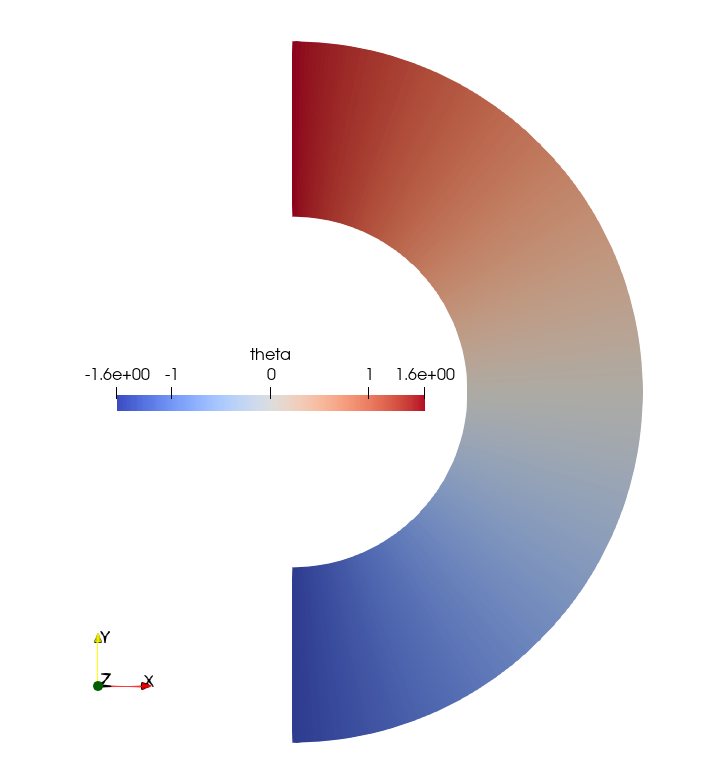
\includegraphics[width=8.3cm]{images/theta}
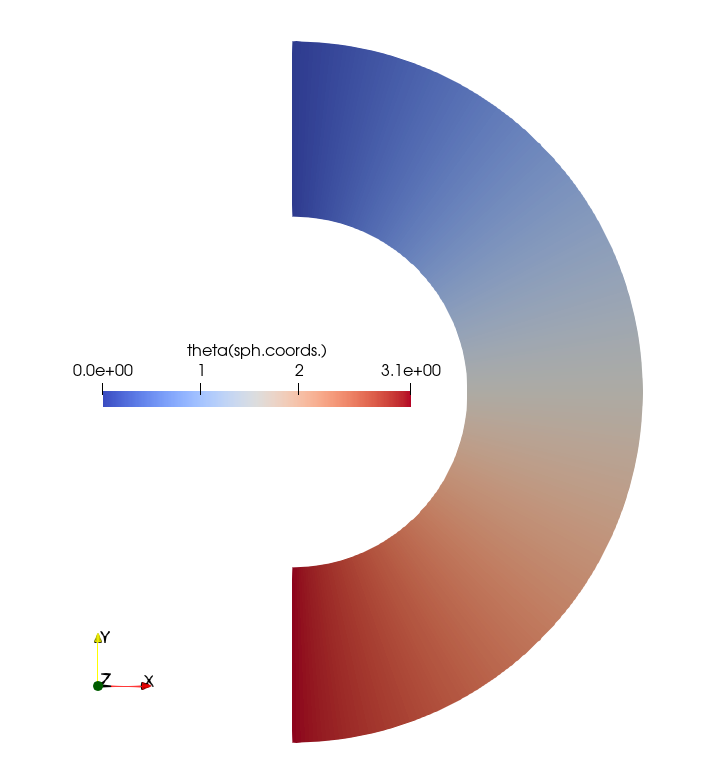
\includegraphics[width=8.3cm]{images/theta_sph}
\end{center}

\begin{lstlisting}
for i in range(0,NV):
    theta_sph[i]=np.pi/2-math.atan(yV[i]/abs(xV[i]))
    if xV[i]>=0:
       e_rr[i]=exx2[i]*np.sin(theta_sph[i])**2+\
               2*exy2[i]*np.sin(theta_sph[i])*np.cos(theta_sph[i])+\
               eyy2[i]*np.cos(theta_sph[i])**2
       e_tt[i]=exx2[i]*np.cos(theta_sph[i])**2-\
               2*exy2[i]*np.sin(theta_sph[i])*np.cos(theta_sph[i])+\
               eyy2[i]*np.sin(theta_sph[i])**2
       e_rt[i]=(exx2[i]-eyy2[i])*np.sin(theta_sph[i])*np.cos(theta_sph[i])+\
               exy2[i]*(-np.sin(theta_sph[i])**2+\
               np.cos(theta_sph[i])**2)
\end{lstlisting}





%----------------------------------------------------------
\subsection{Dynamic topography}


Looking at the ASPECT manual, we find:

``we evaluate the stress and evaluate the component of it in the direction in which 
gravity acts. In other words we compute 
\[
\sigma_{rr}={\hat g}^T (2 \eta \varepsilon(\mathbf u)
- \frac 13 (\textrm{div}\;\mathbf u)I)\hat g - p_d
\] 
where 
$\hat g = \mathbf g/\|\mathbf g\|$ is the direction of 
the gravity vector $\mathbf g$ and $p_d=p-p_a$ is the dynamic 
pressure computed by subtracting the adiabatic pressure $p_a$ 
from the total pressure $p$ computed as part of the Stokes 
solve. From this, the dynamic 
topography is computed using the formula 
\[
h=\frac{\sigma_{rr}}{(\mathbf g \cdot \mathbf n)  \rho}
\] 
where $\rho$ is the density. For the bottom surface we chose the convection 
that positive values are up (out) and negative values are in (down), analogous to 
the deformation of the upper surface. 
The file format then consists of lines with Euclidean coordinates 
followed by the corresponding topography value.''

Here the viscosity is constant in the domain, the flow 
is incompressible and $\vec{g}= -g_0 \vec{e}_r$ so we can compute the 
dynamic topography as follows:
\[
h = - \frac{-p + 2 \eta_0 \dot{\varepsilon}_{rr} }{\rho_0 g_0}
\]
This is of course valid if what is above the surface is a fluid with zero density.
This translates into:

\begin{lstlisting}
dyn_topo=np.zeros(NV,dtype=np.float64)
for i in range(0,NV):
    if surfaceV[i] and xV[i]>=0:
       dyn_topo[i]= -(2*viscosity*e_rr[i]-q[i])/(rho0*g0) 
\end{lstlisting}

Note that in our case $\rho_0=1$ and $g_0=1$ so that in fact the dynamic topography 
is simply $-\sigma_{rr}$.








%%%%%%%%%%%%%%%%%%%%%%%%%%%%%%%%%%%%%%%%%%%%%%%%%%%%%%%%%%%%%%%%%%%%%%%%%%%%%%%
\newpage
\section{Numerical methods}

%----------------------------------------------------------
\subsection{Finite elements}
The discretisation of the Stokes equations by means of the Finite Element Method
is presented in Chapter 5 of fieldstone. Numerical quadrature is explained in 
Section 3.1 and two-dimensional basis functions in Section 3.4.
Note that the special case of cylindrical axisymmetry is discussed in Section 5.4.3.


%----------------------------------------------------------
\section{Nomenclature}

\begin{itemize}
\item Mesh \& geometry
\begin{itemize}
\item {\python nelr}: number of elements in the radial direction  (integer)
\item {\python nelt}: number of elements in the tangential direction (integer)
\item {\python xi}: ratio of {\python nelt} and {\python nelr} (integer)
\item {\python nel}: total number of elements (integer)
\item {\python NV}: number of velocity nodes (integer)
\item {\python NP}: number of pressure nodes (integer)
\item {\python xV,zV}: coordinates of velocity nodes (float64 array size {\python NV}) 
\item {\python xP,zP}: coordinates of pressure nodes (float64 array size {\python NP}) 
\item {\python xc,zc}: coordinates of element centers (float64 array size {\python nel}) 
\item {\python rad,theta}: $r$ and $\theta$ spherical coordinates of velocity nodes  (float64 array size {\python NV}) 
\item {\python nx,ny}: 
\item {\python u,v}: velocity field (float64 array size {\python NV})
\item {\python p}: pressure field (float64 array size {\python NP})
\item {\python q}: pressure field projected on velocity nodes (float64 array size {\python NV})
\end{itemize}
\item Finite elements
\begin{itemize}
\item {\python mV}: number of velocity nodes per element (integer)
\item {\python mP}: number of pressure nodes per element (integer)
\item {\python ndofV}: number of velocity dof per node (integer) 
\item {\python ndofP}: number of pressure dof per node (integer) 
\item {\python NfemV}: total number of velocity dofs (integer) 
\item {\python NfemP}: total number of pressure dofs  (integer) 
\item {\python Nfem}: total number of dofs  (integer) 
\item {\python iconV}: connectivity array for velocity nodes (integer array) 
\item {\python iconP}: connectivity array for pressure nodes (integer array)
\item {\python bc\_fix}: (boolean array size {\python NfemV})
\item {\python bc\_val}: (float 64 array size {\python NfemV})
\end{itemize}
\item Mapping
\begin{itemize}
\item {\python mapping}: type of mapping ({\python 'Q1','Q2','Q3','Q4','Q5','Q6'}) 
\item {\python mmapping}: number of support points ({\python 4,9,16,25,36,49})
\item {\python xmapping}: $x$-coordinates of all mapping support points, array ({\python mmapping},{\python nel}) 
\item {\python zmapping}: $z$-coordinates of all mapping support points, array ({\python mmapping},{\python nel}) 
\item {\python jcb}: Jacobian matrix (float64 array, size (2,2))
\item {\python jcbi}: inverse of Jacobian matrix (float64 array, size (2,2))
\item {\python jcob}: determinant of Jacobian matrix 
\end{itemize}
\item Quadrature
\begin{itemize}
\item {\python nqperdim}: number of quadrature points in 1D
\item {\python nqel}: number of quadrature points pr element ({\python nqperdim**2})
\item {\python qcoords\_r}: $r$-coordinates of the {\python nqel} quadrature points (float 64 array)
\item {\python qcoords\_s}: $s$-coordinates of the {\python nqel} quadrature points  (float 64 array)
\item {\python qweights}: associated weights of the {\python nqel} quadrature points  (float 64 array)
\item {\python xq}: $x$-coordinates of all quadrature points (float64 array size ({\python nel*nqel})) 
\item {\python zq}: $z$-coordinates of all quadrature points (float64 array size ({\python nel*nqel})) 
\end{itemize}

\end{itemize}






%----------------------------------------------------------
\subsection{Mapping}


After discretising the domain in {\python nel} elements, and having decided the FE
pair we want to use to solve the Stokes equations (in this case \QtwoQone), we end up 
having to compute elemental integrals such as 
\[
\K_e = \int_{\Omega_e} {\bm B}^T\cdot {\bm C}_\eta \cdot {\bm B} \; d\Omega
\]
where $\Omega_e$ denotes an element.
The way we carry out this integration is by means of the Gauss-Legendre quadrature
(see Section~\ref{MMM-sec:quadrature}), which 
forces us to carry out a change of variables from the original element $\Omega_e$ 
to the reference element $(r,s) \in [-1,1]\times [-1,1]$. For this we establish a mapping between both 
as explained in Section~\ref{MMM-ss:mappings}.
Basis functions $Q_{1,2,3,4}$ are defined in Section~\ref{MMM-sec:shpfct2d}.

\begin{center}
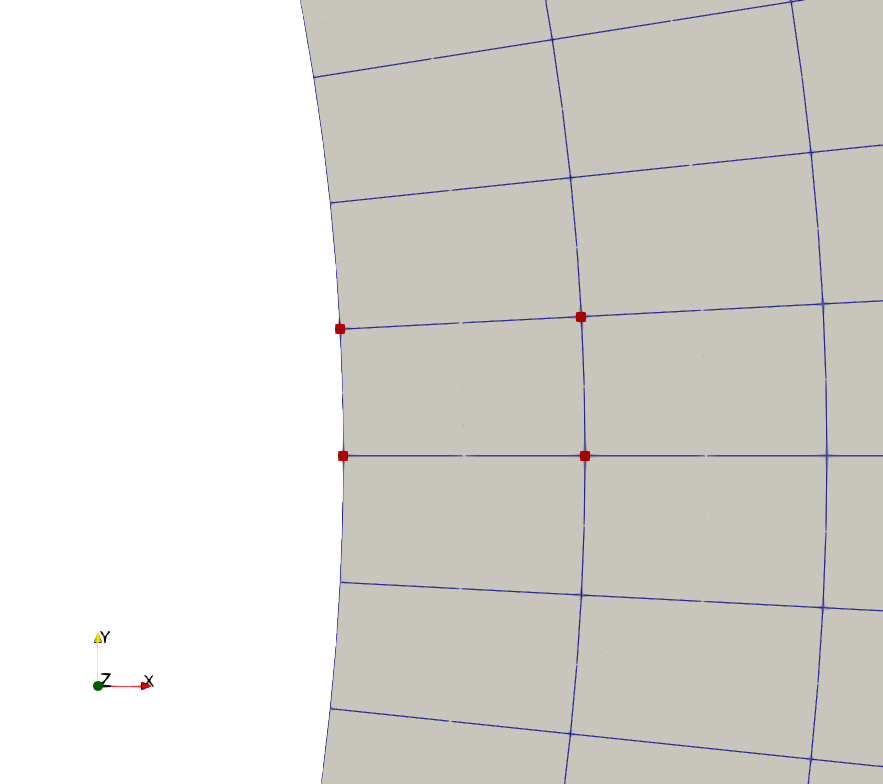
\includegraphics[width=4.2cm]{images/mappingQ1}
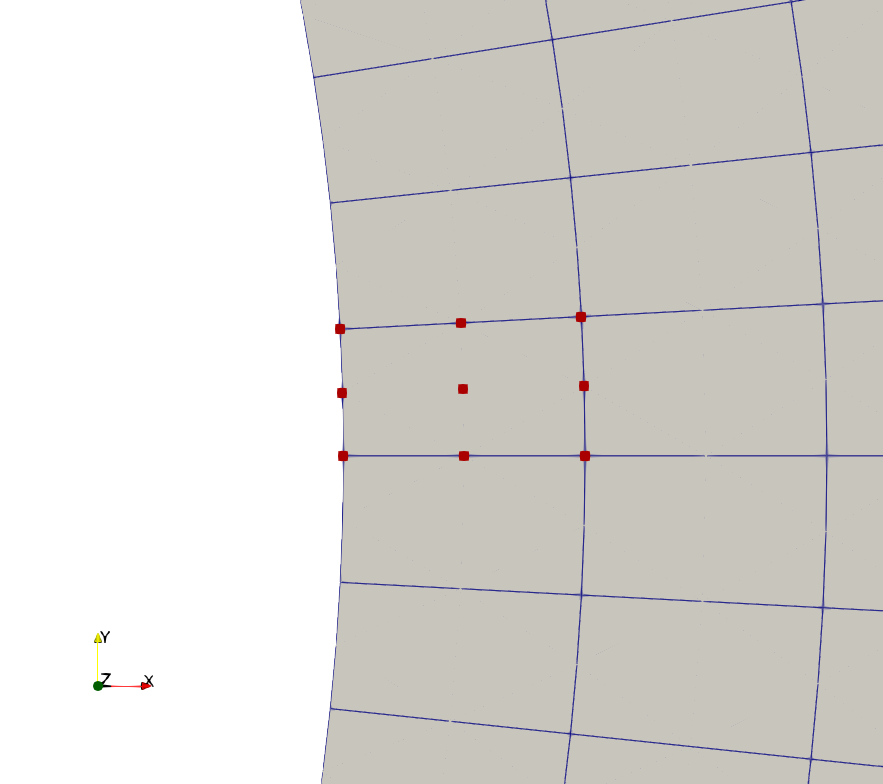
\includegraphics[width=4.2cm]{images/mappingQ2}
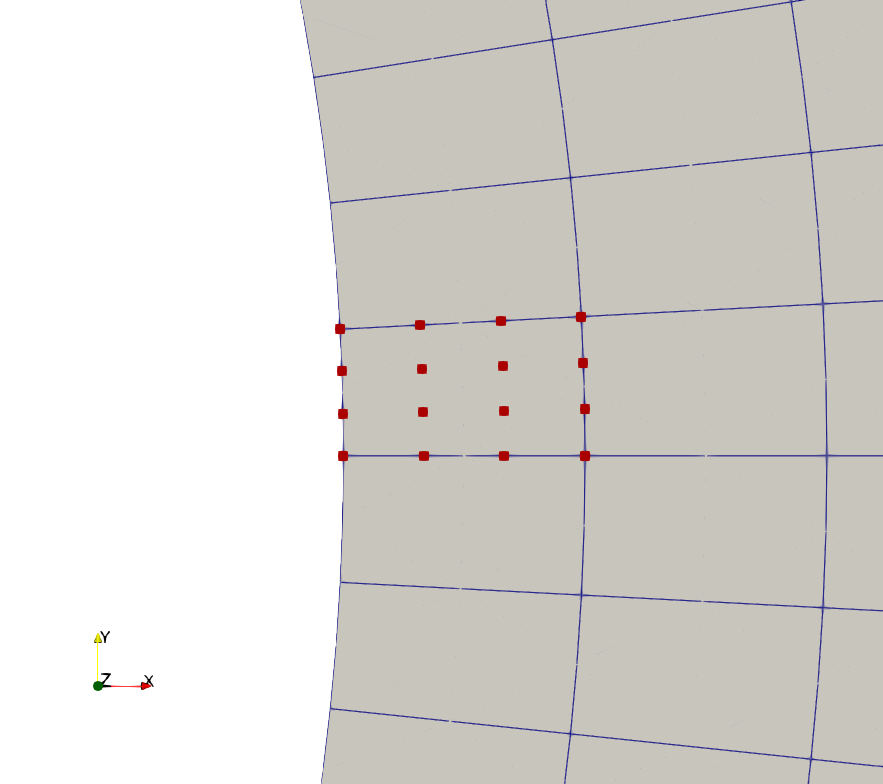
\includegraphics[width=4.2cm]{images/mappingQ3}
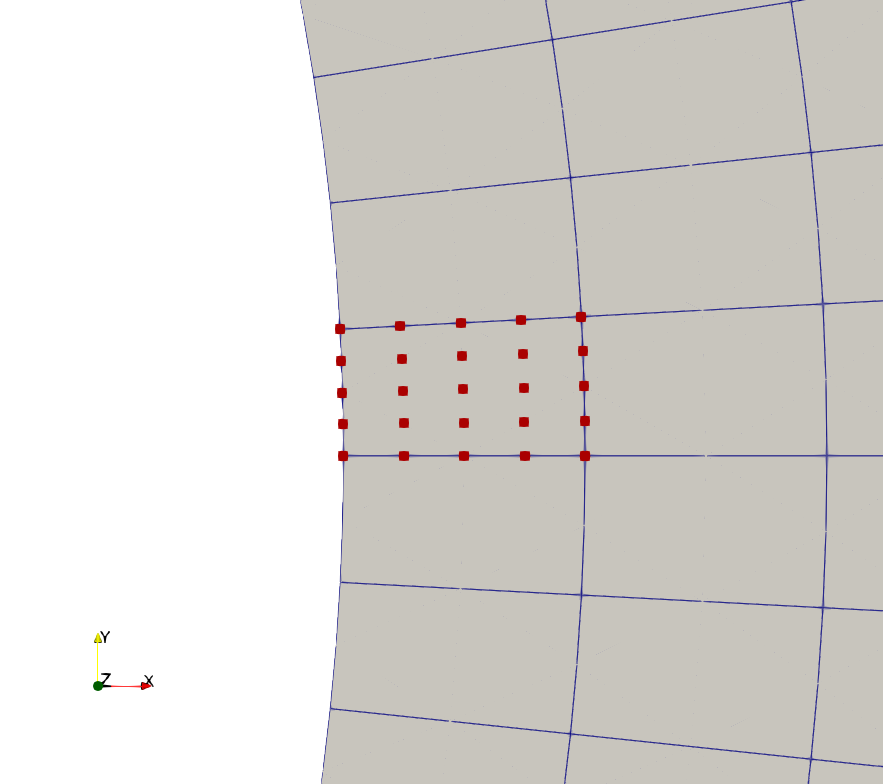
\includegraphics[width=4.2cm]{images/mappingQ4}\\
{\captionfont Layout of the mapping nodes in element \#0 of the mesh. 
From left to right: $Q_1$, $Q_2$, $Q_3$ and $Q_4$. Rows of nodes are placed 
on concentric circles and columns of nodes are equidistant in $\theta$ space.} 
\end{center}

For each element we store the coordinates of these mapping points into two 
arrays:
\begin{lstlisting}
xmapping=np.zeros((X,nel),dtype=np.float64)
ymapping=np.zeros((X,nel),dtype=np.float64)
\end{lstlisting}
where {\python X} stands for the number of nodes for each mapping.

The reduced coordinates for the quadrature points are given by 
the Gauss-Legendre quadrature approach. The real coordinates of these points
is a function of the mapping used so that 
\begin{lstlisting}
for iel in range(0,nel):
    for kq in range(0,nqel):
        rq=qcoords_r[kq]
        sq=qcoords_s[kq]
        NNNV=NNN(rq,sq,mapping)
        xq=np.dot(NNNV[:],xmapping[:,iel])
        yq=np.dot(NNNV[:],ymapping[:,iel])
\end{lstlisting}
Likewise the Jacobian matrix is by definition a function of the chosen mapping 
so that 
\begin{lstlisting}
for iel in range(0,nel):
    for kq in range(0,nqel):
        rq=qcoords_r[kq]
        sq=qcoords_s[kq]
        dNNNVdr=dNNNdr(rq,sq,mapping)
        dNNNVds=dNNNds(rq,sq,mapping)
        jcb[0,0]=np.dot(dNNNVdr[:],xmapping[:,iel])
        jcb[0,1]=np.dot(dNNNVdr[:],ymapping[:,iel])
        jcb[1,0]=np.dot(dNNNVds[:],xmapping[:,iel])
        jcb[1,1]=np.dot(dNNNVds[:],ymapping[:,iel])
        jcob=np.linalg.det(jcb)
        jcbi=np.linalg.inv(jcb)
\end{lstlisting}


\begin{center}
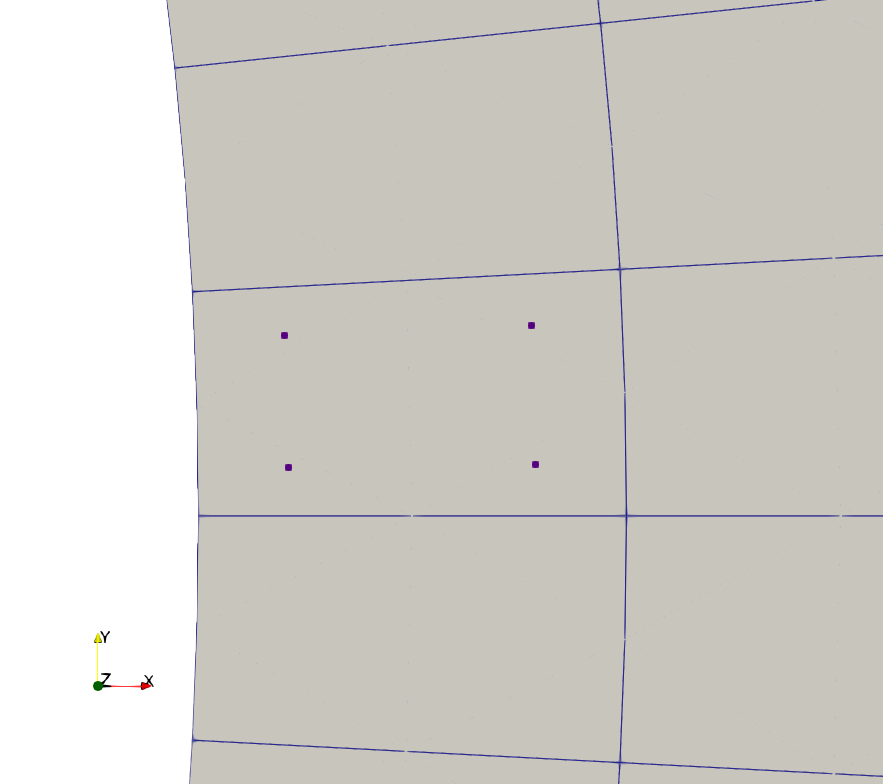
\includegraphics[width=4.2cm]{images/nq4}
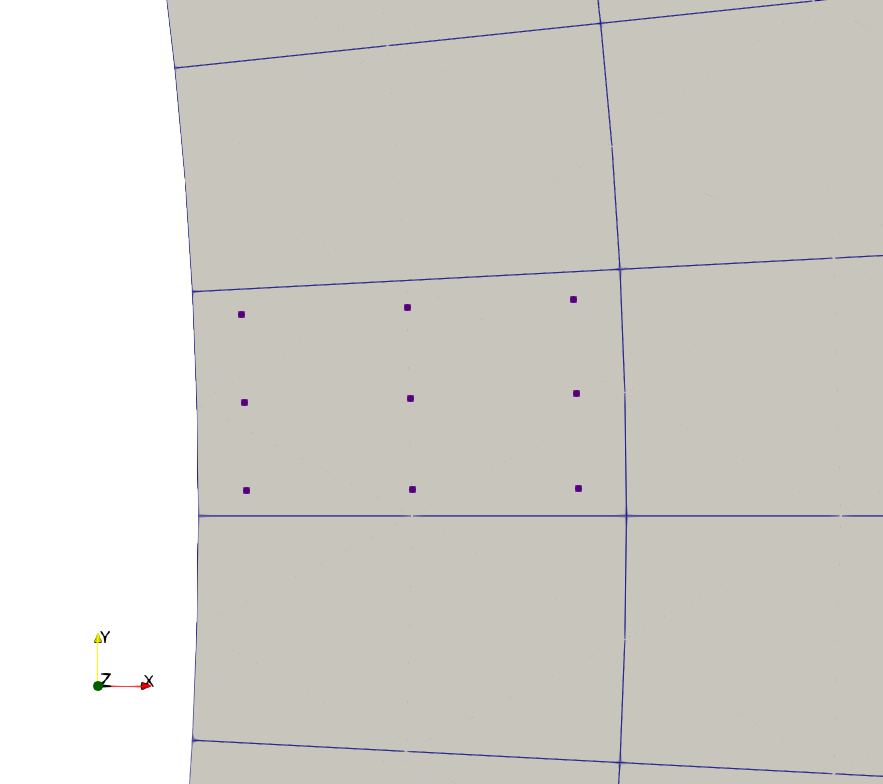
\includegraphics[width=4.2cm]{images/nq9}
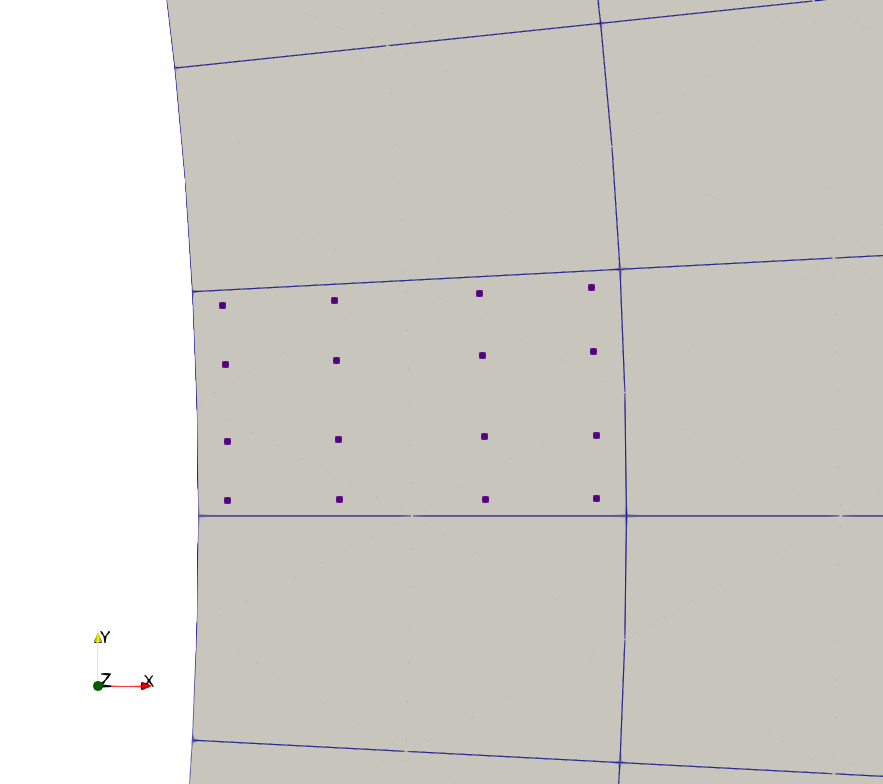
\includegraphics[width=4.2cm]{images/nq16}
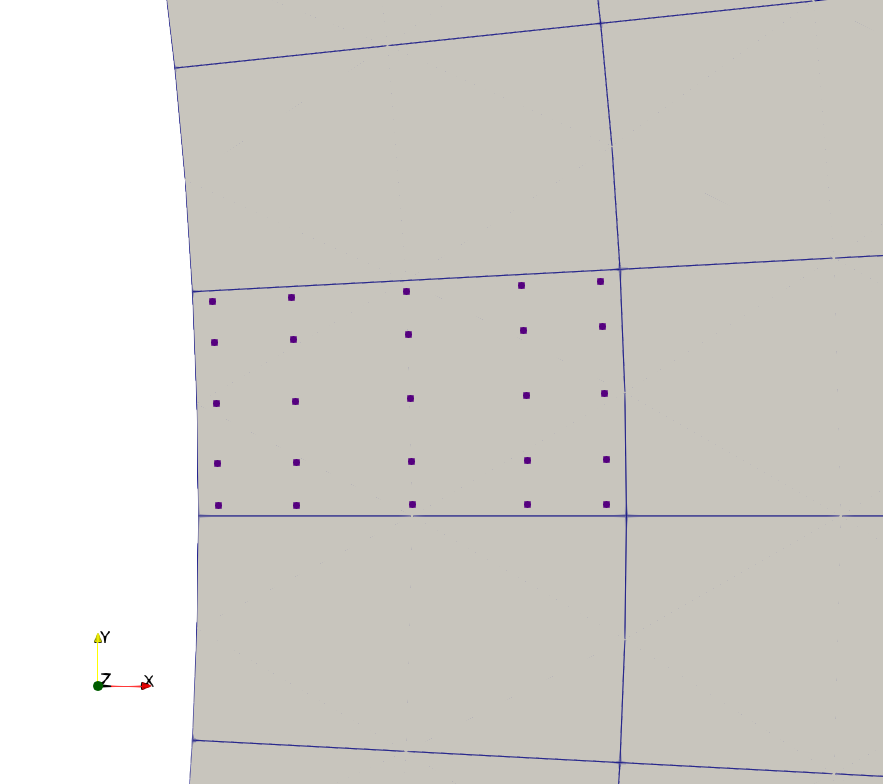
\includegraphics[width=4.2cm]{images/nq25}\\
{\captionfont Layout of the quadrature points in element \#0 of the mesh. 
From left to right: {\python nqperdim=2,3,4,5}.} 
\end{center}

Note that the {\python axisymmetric} flag controls whether the Stokes equations 
are solved in plane strain or under the assumption that there is axisymmetry. 
In the latter case the mesh is a demi-annulus in the $x>0$ half plane.



%----------------------------------------------------------
\subsection{Quadrature}

%----------------------------------------------------------
\subsection{Computing normals}

- axisymmetric case only

As seen in stone~\ref{f151}, there are (at least) two ways to compute the normal at the
nodes on the surface: $\vec{n}_1$ which is purely geometric and $\vec{n}_2$ which is based 
on an integration of the basis function derivatives.
We found that in the case of the annulus the two coincided to machine precision. 
Let us now turn the half annulus. As an experiment, {\it all} nodes on the hull are flagged
and the normal $\vec{n}_2$ is computed. 
Since this normal is a function of basis functions and requires an integration 
over elements, we can ask ourselves whether the mapping and/or the number
of quadrature points influence the results of the normal calculations.
The {\tt script\_normals} bash script runs the required models - note that the
$Q_1$ mapping and nqperdim=2 have been removed from the loops.

\begin{center}
\includegraphics[width=8cm]{RESULTS/normals/nx}
\includegraphics[width=8cm]{RESULTS/normals/ny}\\
\includegraphics[width=8cm]{RESULTS/normals/nnx}
\includegraphics[width=8cm]{RESULTS/normals/nny}\\
{\captionfont components of the normal vector on the hull (first line),
on the surface (second line). Mesh is 8x96.}
\end{center}

We find that these normal vector components do not seem to depend on the mapping nor quadrature,
and that on the curved parts they match their geometrical counterparts $\vec{n}_1$.
These normal vectors are shown here:

\begin{center}
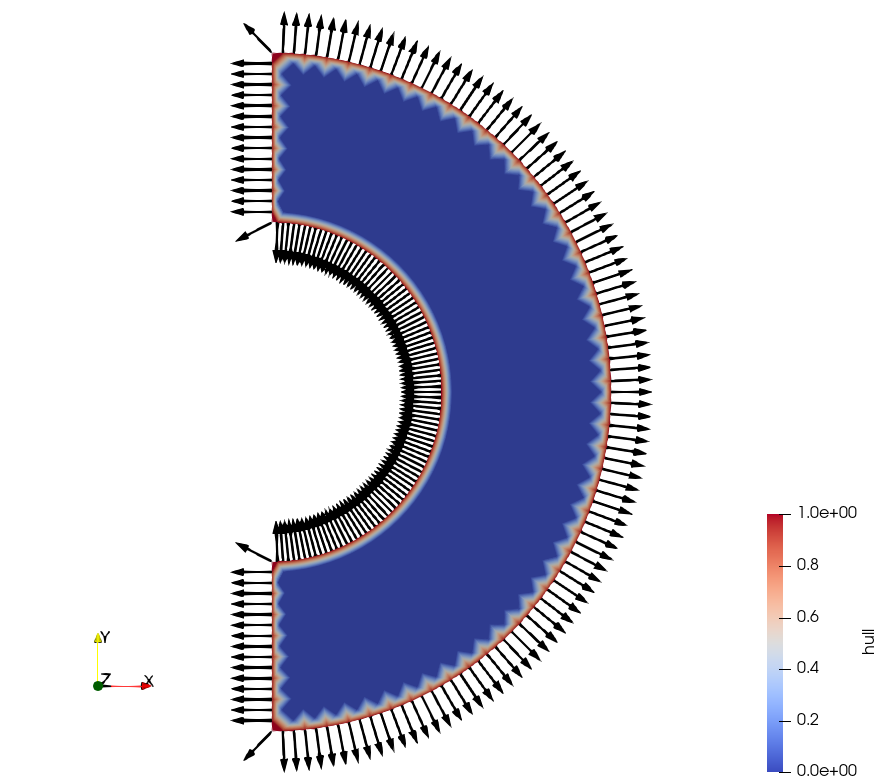
\includegraphics[width=6cm]{RESULTS/normals/normals}
\end{center}

Obviously, we need to look closer at the four nodes that belong to the surface and the cmb with $x=0$.
On the one hand they belong the vertical boundary $x=0$ so their horizontal velocity component should be zero (axisymmetry).
On the other hand they also belong to the curved boundaries. In the case of a near infinite resolution the 
normal to the curved part would align with the vertical axis so that we would then have $v=0$. 
In the end these 4 points should be prescribed no-slip boundary conditions.

In our case here only the surface can be prescribed free slip boundary conditions and there are {\python nnt} points at the surface.
Removing the 2 extremities, we have {\python nnt-2} Lagrange multipliers. Note that then how we compute normals is not relevant.

\begin{center}
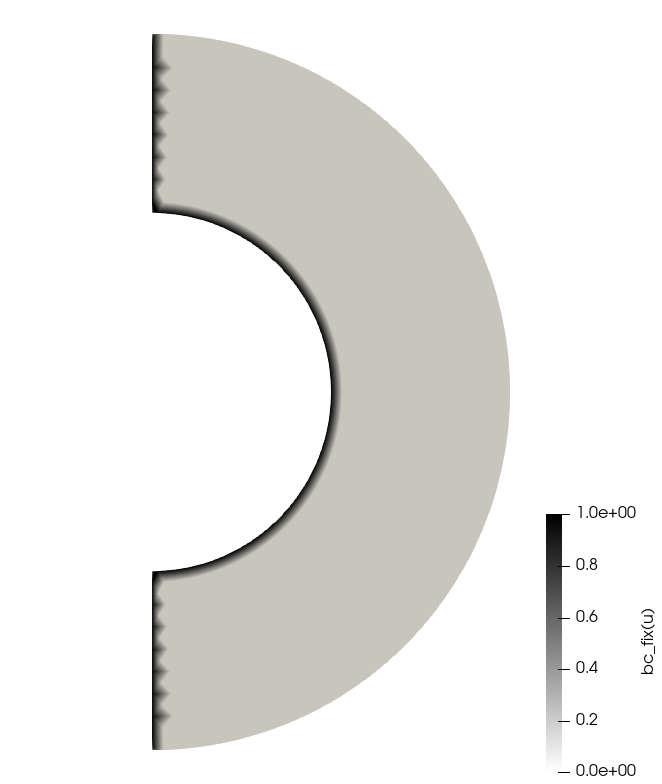
\includegraphics[width=6cm]{images/bcfix_u}
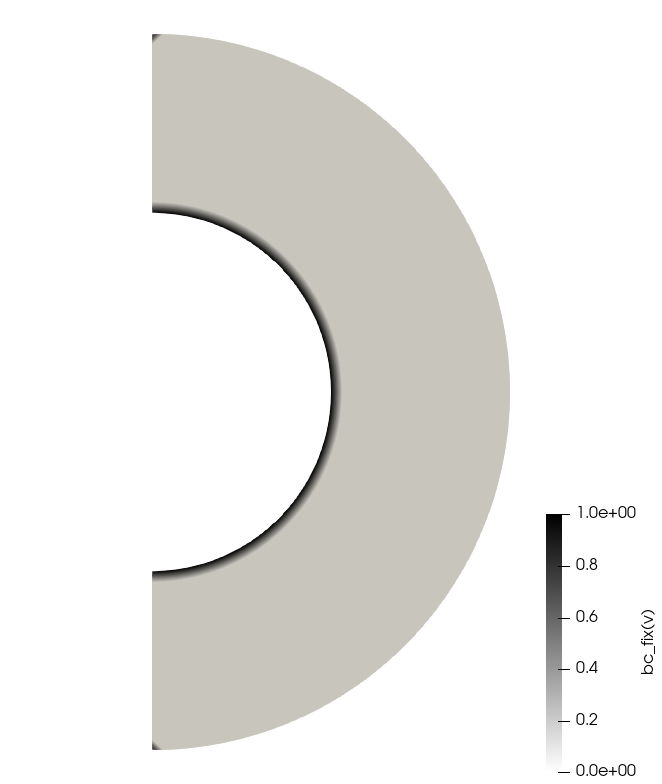
\includegraphics[width=6cm]{images/bcfix_v}\\
{\captionfont horizontal and vertical boundary condition indicators.}
\end{center}




%----------------------------------------------------------
\subsection{Implementing free slip boundary conditions}


Finally free slip boundary conditions have been implemented, but only at the 
surface, and only with the method of Lagrange Multipliers (\stone~\ref{f151}
taught us that it works as well as the other method).  
{\color{red} change}

\begin{eqnarray}
\K_e \cdot \vec{\cal V} + \G_e \cdot \vec{\cal P} &=& \vec{f}  \\
\G_e \cdot \vec{\cal V} &=& \vec{0}
\end{eqnarray}
We multiply the first line by the rotation matrix ${\bm R}$:
\begin{eqnarray}
{\bm R} \cdot \K_e \cdot \vec{\cal V} +{\bm R} \cdot \G_e \cdot \vec{\cal P} &=&{\bm R} \cdot \vec{f}  \\
\G_e \cdot \vec{\cal V} &=& \vec{0}
\end{eqnarray}
and then introduce the identity matrix ${\bm I}={\bm R}^T\cdot {\bm R}$ before the velocity vector:
\begin{eqnarray}
{\bm R} \cdot \K_e \cdot {\bm R}^T\cdot {\bm R} \cdot  \vec{\cal V} +{\bm R} \cdot \G_e \cdot \vec{\cal P} &=&{\bm R} \cdot \vec{f}  \\
\G_e \cdot  {\bm R}^T\cdot {\bm R} \cdot  \vec{\cal V} &=& \vec{0}
\end{eqnarray}
The second line can also be written
\begin{eqnarray}
({\bm R} \cdot \K_e \cdot {\bm R}^T) \cdot ({\bm R} \cdot  \vec{\cal V}) + ({\bm R} \cdot \G_e) \cdot \vec{\cal P} &=&{\bm R} \cdot \vec{f}  \\
( {\bm R} \cdot \G_e)^T \cdot  ({\bm R} \cdot  \vec{\cal V}) &=& \vec{0}
\end{eqnarray}
which translates at the elemental level into
\begin{lstlisting}
K_el=RotMat.dot(K_el.dot(RotMat.T))
f_el=RotMat.dot(f_el)
G_el=RotMat.dot(G_el)
\end{lstlisting}
Note that the matrix $\K_e$ is $(m*ndofV)\times (m*ndofV)$ in size, and so is the matrix ${\bm R}$.

After boundary conditions are imposed, the system is rotated back:

\begin{lstlisting}
K_el=RotMat.T.dot(K_el.dot(RotMat))
f_el=RotMat.T.dot(f_el)
G_el=RotMat.T.dot(G_el)
\end{lstlisting}


%----------------------------------------------------------
\subsection{Pressure normalisation}

%-------------------------
\subsubsection*{Plane strain}

In polar coordinates the surface element is 
\[
dS = R d\theta
\]
so that 
$\int_0^{2\pi} dS = \int_0^{2\pi} R d\theta = 2 \pi R$ which is the perimeter of the circle.

We wish to normalise the pressure so that it is on average zero on the surface:
\[
p_{normalised} = p - <p>
\]
where 
\[
<p> 
= \frac{\int p(r, \theta) dS }{\int dS}
= \frac{\int p(\theta) R d\theta }{\int R d \theta d\theta}
= \frac{1}{2 \pi R} R \int p(\theta) d\theta 
= \frac{1}{2 \pi }  \int_0^{2\pi} p(\theta) d\theta 
\]
This integral is broken up in a summation over element edges which are at the surface.
\[
<p>= \frac{1}{2\pi} \sum_{e}^{nelt} \int_{\theta_{2}^e}^{\theta_{3}^e} p (\theta) d\theta
\]
where $\theta_2^e$ and $\theta_3^e$ are the $\theta$ values of nodes 2 and 3 of element $e$ that lie on the surface.
These edge integrals are simplifed by assuming a 1-point quadrature:
\[
<p>= \frac{1}{2\pi} \sum_{e}^{nelt}  p (\frac{\theta_2^e+\theta_3^e}{2}) (\theta_3^e-\theta_2^e)
\]



%------------------------------
\subsubsection*{Axisymmetric case}

\begin{center}
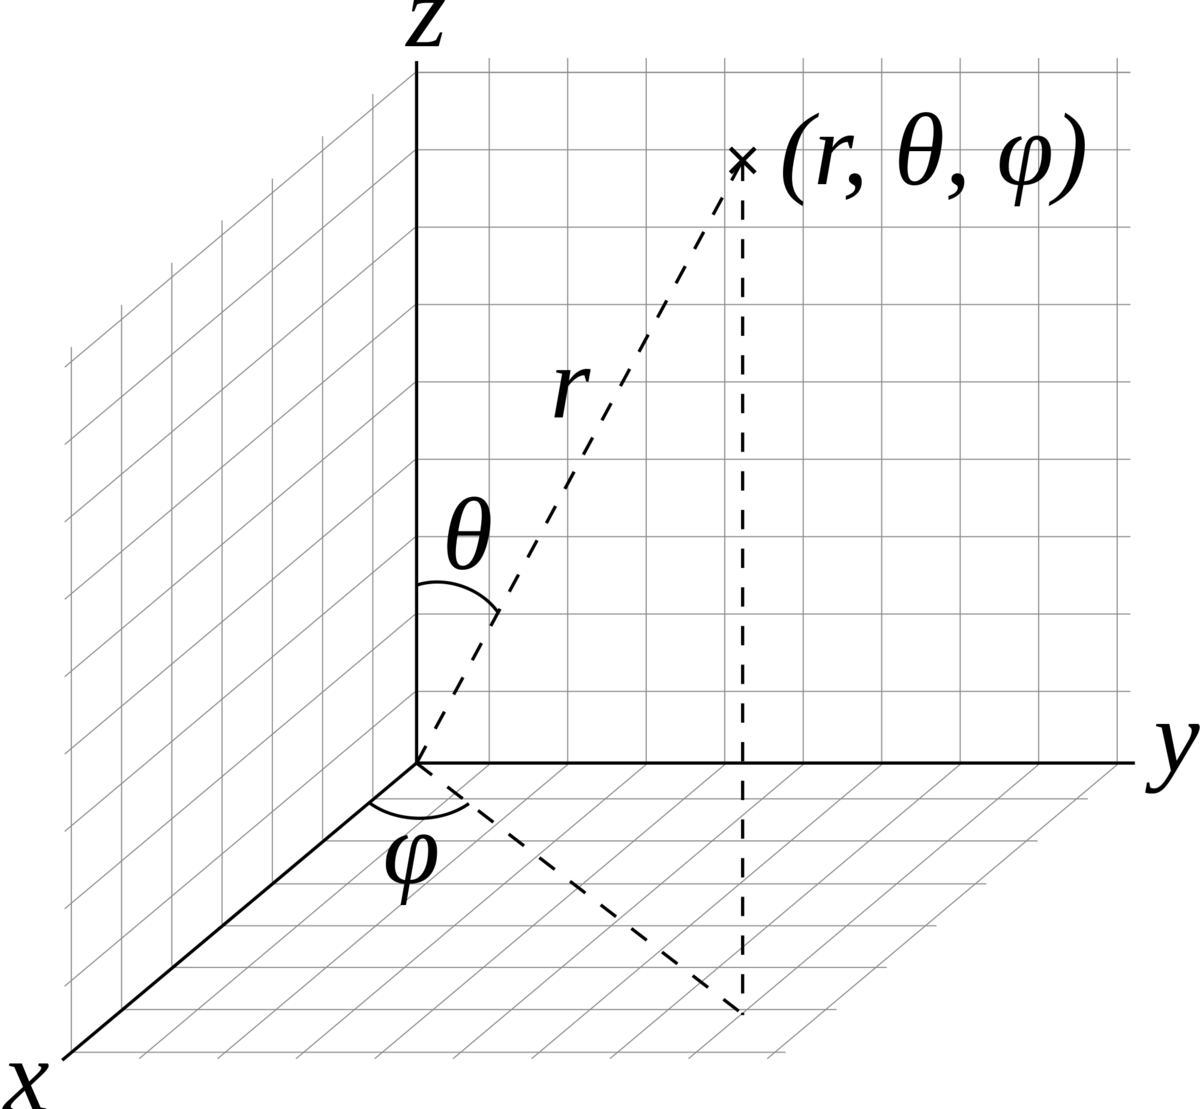
\includegraphics[width=3cm]{images/sphcoord}
\end{center}

In spherical coordinates, the surface element is 
\[
dS= R^2 \sin \theta d\theta d\phi
\]
We wish to normalise the pressure so that it is on average zero on the surface:
\[
p_{normalised} = p - <p>
\]
where 
\[
<p> 
= \frac{\iint p(\theta,\phi) dS }{\iint dS}
= \frac{\iint p(\theta,\phi) R^2 \sin \theta d\theta d\phi}{\iint R^2 \sin \theta d\theta d\phi}
\]
and since $p$ is independent of $\phi$ then 
\[
<p> 
= \frac{R_2^2 \cdot 2\pi \cdot  \int_0^\pi p(\theta)  \sin \theta d\theta}
{R_2^2 \cdot 2\pi \cdot \int  \sin \theta d\theta }
= \frac{ 2\pi R_2^2 \int_0^\pi p(\theta)  \sin \theta d\theta} {4\pi R_2^2}
\]
The integral over $\theta$ can be simplified by using the average pressure 
along the edge and the angle of the edge middle point:
\begin{lstlisting}
poffset=0
for iel in range(0,nel):
    if surface_element[iel]:
       dtheta=theta_sph[iconV[2,iel]]-theta_sph[iconV[3,iel]]
       pmean=0.5*(p[iconP[2,iel]]+p[iconP[3,iel]])
       poffset+=np.sin((theta_sph[iconV[2,iel]]+theta_sph[iconV[3,iel]])/2)*dtheta\
                *2*np.pi*R2**2 * pmean
poffset/=4*np.pi*R2**2
\end{lstlisting}




%%%%%%%%%%%%%%%%%%%%%%%%%%%%%%%%%%%%%%%%%%%%%%%%%%%%%%%%%%%%%%%%%%%%%%%%%%%%%%%
\newpage
\section{The data}

%----------------------------------------------------------
\subsection{Earth}

We assume that viscosity is purely a function of depth\footnote{This is borrowed
from stone 71}.. 

Five radial viscosity profiles are available:
\begin{itemize}
\item The first viscosity profile is a constant viscosity for all depths of $10^{22}$ Pa s.
This value is an estimated value of what is normally found in the literature. 

\item The second viscosity profile comes from Yoshida et al (2001) \cite{yohk01}. It uses three different regions: lithosphere (0 km to 150 km), upper mantle (150 km to 670 km) and lower mantle (670 km to 2900 km).

\item The third viscosity profile comes from Steinberger \& Holmes (2008) \cite{stho08}
which is comparable to \cite{stca06}, but of the latter no available data was available.
Data is read from the file \texttt{DATA/EARTH/eta\_stho08.ascii}.

\item The fourth and fifth profile come from Ciskova et al (2012) \cite{civs12}.
Data is read from the file \texttt{DATA/EARTH/eta\_civs.ascii}.
The paper showcases two main families of radial viscosity profiles in literature. Family A, which has a sharp
increase below the 660 km transition zone and remains constant for most of the lower mantle
and family B which is much smoother over the transition zone and increases with depth in the lower mantle.

\end{itemize}

Three radial density profiles are available:

\begin{itemize}
\item PREM \cite{dzan81}
\item ak135f \cite{keeb95} \url{http://rses.anu.edu.au/seismology/ak135/ak135f.html}
Data is read from the file \texttt{DATA/EARTH/rho\_ak135f.ascii}.
\item stw105 \cite{kued08} \url{http://ds.iris.edu/ds/products/emc-stw105/}
Data is read from the file \texttt{DATA/EARTH/rho\_stw105.ascii}.
\end{itemize}



%----------------------------------------------------------
\subsection{Mars}


%%%%%%%%%%%%%%%%%%%%%%%%%%%%%%%%%%%%%%%%%%%%%%%%%%%%%%%%%%%%%%%%%%%%%%%%%%%%%%%
\newpage
\section{Benchmarking}



The goal here is to explore the influence of the mapping polynomial order and/or
the number of quadrature points on the accuracy of the solution of various benchmarks and test cases.

Concretely, in this section we will explore the effect of:
\begin{itemize}
\item resolution via the number of elements in the radial direction: {\python nelr=2-32} (we automatically set {\python nelt=12*nelr})
\item the number of quadrature points per dimension: {\python nqperdim=2,3,4,5}
\item the polynomial order of the mapping: {\python mapping='Q1','Q2','Q3','Q4'}
\end{itemize}
and we will monitor the computed area/volume, the root mean square velocity and the velocity and pressure errors.

\subsection{Computing volume/mass}

Here we simply compute 
\[
{\cal V} = \sum_e \int_{\Omega_e} 2\pi x dV
\]
where the sum runs over all elements of the domain.
We of course have 
\[
{\cal V}_{analytical} = \frac43 \pi (R_2^3-R_1^3)
\]
so that we can compute the relative errors as a function of resolution, mapping and quadrature: 
\begin{center}
\includegraphics[width=12cm]{RESULTS/vols/volumes.pdf}
\end{center}

\noindent Conclusions:
\begin{itemize}
\item unsurprisingly $Q_1$ mapping yields the worst results
\item mapping is the controling factor, much more than quadrature
\item for the isoparametric element (mapping $Q_2$) the number of quadrature points 
is not critical. Results are virtually identical for {\python nqperdim=2,3,4,5}
\item $Q_3$ about one order of magnitude more accurate than $Q_2$ 
\item $Q_4$ mapping 3-4 orders of magnitude more accurate than $Q_2$ mapping
\end{itemize}




\subsection{Annulus convection manufactured solution}


%%%%%%%%%%%%%%%%%%%%%%%%%%%%%%%%%%%%%%%%%%%%%%%%%%%%%%%%%%%%%%%%%%%%%%%%%%%%%%%
\section{The '4D dynamic earth' inter-code benchmark}

\cite{krhb12}


%%%%%%%%%%%%%%%%%%%%%%%%%%%%%%%%%%%%%%%%%%%%%%%%%%%%%%%%%%%%%%%%%%%%%%%%%%%%%%%
%%%%%%%%%%%%%%%%%%%%%%%%%%%%%%%%%%%%%%%%%%%%%%%%%%%%%%%%%%%%%%%%%%%%%%%%%%%%%%%
\newpage
\appendix
\section{Misc}

%----------------------------------------------------------
\subsection{Notes to self}

What I have tried to cure the pb of the weird anomalies at the poles.

\begin{itemize}
\item turning elements into real trapezes. Made things worse
\item different mappings. not much difference
\item when using blob, reduced densities. no difference
\item nb of quad points, no real difference
\item nb of elements in tangential direction, some difference but no cure 
\item when using blob, drho/rho, no diff 
\item type of b.c. at point corner below poles, no real diff 
\item scaling of G matrix
\item different rotations/bc for free slip, no difference
\item using cmat matrix for dev strain rate, helped a little bit, no cure 
\end{itemize}



%----------------------------------------------------------
\subsection{To do list}
\begin{itemize}
\item visc profiles
\item rho profiles
\item time stepping
\item gravity calculations. import from f96, re-benchmark
\item CBF? 
\item compute self gravity for reduced density case 
\item export exx1 and exx3 to outside function, clean their code too? 
\item remove call to math 
\item bottom free slip 
\item change y for z in stone
\item use PREM gravity value
\item aspect with GMG ?
\item compute moment of inertia
\item by default code now uses elemental rho and eta. it changes things wrt exp0 benchmark results!
\item change all eyy and exy to ezz exz
\end{itemize}




\bibliography{bibliography} 

\end{document}
%%%%%%%%%%%%%%%%%%%%%%%%%%%%%%%%%%%%%%%%%%%%%%%%%%%%%%%%%%%%%%%%%%%%%%%%%%%%%%%
